\documentclass[10pt,a4paper]{article}
\usepackage{ucs}
\usepackage[a4paper,top=2cm,bottom=2cm,left=3cm,right=3cm,marginparwidth=1.75cm]{geometry}

\usepackage[utf8x]{inputenc}
\usepackage[hebrew, english]{babel}
\usepackage{culmus}
%%%%% NEW MATH DEFINITIONS %%%%%

\usepackage{amsmath,amsfonts,bm}

% Mark sections of captions for referring to divisions of figures
\newcommand{\figleft}{{\em (Left)}}
\newcommand{\figcenter}{{\em (Center)}}
\newcommand{\figright}{{\em (Right)}}
\newcommand{\figtop}{{\em (Top)}}
\newcommand{\figbottom}{{\em (Bottom)}}
\newcommand{\captiona}{{\em (a)}}
\newcommand{\captionb}{{\em (b)}}
\newcommand{\captionc}{{\em (c)}}
\newcommand{\captiond}{{\em (d)}}

% Highlight a newly defined term
\newcommand{\newterm}[1]{{\bf #1}}


% Figure reference, lower-case.
\def\figref#1{figure~\ref{#1}}
% Figure reference, capital. For start of sentence
\def\Figref#1{Figure~\ref{#1}}
\def\twofigref#1#2{figures \ref{#1} and \ref{#2}}
\def\quadfigref#1#2#3#4{figures \ref{#1}, \ref{#2}, \ref{#3} and \ref{#4}}
% Section reference, lower-case.
\def\secref#1{section~\ref{#1}}
% Section reference, capital.
\def\Secref#1{Section~\ref{#1}}
% Reference to two sections.
\def\twosecrefs#1#2{sections \ref{#1} and \ref{#2}}
% Reference to three sections.
\def\secrefs#1#2#3{sections \ref{#1}, \ref{#2} and \ref{#3}}
% Reference to an equation, lower-case.
\def\eqref#1{equation~\ref{#1}}
% Reference to an equation, upper case
\def\Eqref#1{Equation~\ref{#1}}
% A raw reference to an equation---avoid using if possible
\def\plaineqref#1{\ref{#1}}
% Reference to a chapter, lower-case.
\def\chapref#1{chapter~\ref{#1}}
% Reference to an equation, upper case.
\def\Chapref#1{Chapter~\ref{#1}}
% Reference to a range of chapters
\def\rangechapref#1#2{chapters\ref{#1}--\ref{#2}}
% Reference to an algorithm, lower-case.
\def\algref#1{algorithm~\ref{#1}}
% Reference to an algorithm, upper case.
\def\Algref#1{Algorithm~\ref{#1}}
\def\twoalgref#1#2{algorithms \ref{#1} and \ref{#2}}
\def\Twoalgref#1#2{Algorithms \ref{#1} and \ref{#2}}
% Reference to a part, lower case
\def\partref#1{part~\ref{#1}}
% Reference to a part, upper case
\def\Partref#1{Part~\ref{#1}}
\def\twopartref#1#2{parts \ref{#1} and \ref{#2}}

\def\ceil#1{\lceil #1 \rceil}
\def\floor#1{\lfloor #1 \rfloor}
\def\1{\bm{1}}
\newcommand{\train}{\mathcal{D}}
\newcommand{\valid}{\mathcal{D_{\mathrm{valid}}}}
\newcommand{\test}{\mathcal{D_{\mathrm{test}}}}

\def\eps{{\epsilon}}


% Random variables
\def\reta{{\textnormal{$\eta$}}}
\def\ra{{\textnormal{a}}}
\def\rb{{\textnormal{b}}}
\def\rc{{\textnormal{c}}}
\def\rd{{\textnormal{d}}}
\def\re{{\textnormal{e}}}
\def\rf{{\textnormal{f}}}
\def\rg{{\textnormal{g}}}
\def\rh{{\textnormal{h}}}
\def\ri{{\textnormal{i}}}
\def\rj{{\textnormal{j}}}
\def\rk{{\textnormal{k}}}
\def\rl{{\textnormal{l}}}
% rm is already a command, just don't name any random variables m
\def\rn{{\textnormal{n}}}
\def\ro{{\textnormal{o}}}
\def\rp{{\textnormal{p}}}
\def\rq{{\textnormal{q}}}
\def\rr{{\textnormal{r}}}
\def\rs{{\textnormal{s}}}
\def\rt{{\textnormal{t}}}
\def\ru{{\textnormal{u}}}
\def\rv{{\textnormal{v}}}
\def\rw{{\textnormal{w}}}
\def\rx{{\textnormal{x}}}
\def\ry{{\textnormal{y}}}
\def\rz{{\textnormal{z}}}

% Random vectors
\def\rvepsilon{{\mathbf{\epsilon}}}
\def\rvtheta{{\mathbf{\theta}}}
\def\rva{{\mathbf{a}}}
\def\rvb{{\mathbf{b}}}
\def\rvc{{\mathbf{c}}}
\def\rvd{{\mathbf{d}}}
\def\rve{{\mathbf{e}}}
\def\rvf{{\mathbf{f}}}
\def\rvg{{\mathbf{g}}}
\def\rvh{{\mathbf{h}}}
\def\rvu{{\mathbf{i}}}
\def\rvj{{\mathbf{j}}}
\def\rvk{{\mathbf{k}}}
\def\rvl{{\mathbf{l}}}
\def\rvm{{\mathbf{m}}}
\def\rvn{{\mathbf{n}}}
\def\rvo{{\mathbf{o}}}
\def\rvp{{\mathbf{p}}}
\def\rvq{{\mathbf{q}}}
\def\rvr{{\mathbf{r}}}
\def\rvs{{\mathbf{s}}}
\def\rvt{{\mathbf{t}}}
\def\rvu{{\mathbf{u}}}
\def\rvv{{\mathbf{v}}}
\def\rvw{{\mathbf{w}}}
\def\rvx{{\mathbf{x}}}
\def\rvy{{\mathbf{y}}}
\def\rvz{{\mathbf{z}}}

% Elements of random vectors
\def\erva{{\textnormal{a}}}
\def\ervb{{\textnormal{b}}}
\def\ervc{{\textnormal{c}}}
\def\ervd{{\textnormal{d}}}
\def\erve{{\textnormal{e}}}
\def\ervf{{\textnormal{f}}}
\def\ervg{{\textnormal{g}}}
\def\ervh{{\textnormal{h}}}
\def\ervi{{\textnormal{i}}}
\def\ervj{{\textnormal{j}}}
\def\ervk{{\textnormal{k}}}
\def\ervl{{\textnormal{l}}}
\def\ervm{{\textnormal{m}}}
\def\ervn{{\textnormal{n}}}
\def\ervo{{\textnormal{o}}}
\def\ervp{{\textnormal{p}}}
\def\ervq{{\textnormal{q}}}
\def\ervr{{\textnormal{r}}}
\def\ervs{{\textnormal{s}}}
\def\ervt{{\textnormal{t}}}
\def\ervu{{\textnormal{u}}}
\def\ervv{{\textnormal{v}}}
\def\ervw{{\textnormal{w}}}
\def\ervx{{\textnormal{x}}}
\def\ervy{{\textnormal{y}}}
\def\ervz{{\textnormal{z}}}

% Random matrices
\def\rmA{{\mathbf{A}}}
\def\rmB{{\mathbf{B}}}
\def\rmC{{\mathbf{C}}}
\def\rmD{{\mathbf{D}}}
\def\rmE{{\mathbf{E}}}
\def\rmF{{\mathbf{F}}}
\def\rmG{{\mathbf{G}}}
\def\rmH{{\mathbf{H}}}
\def\rmI{{\mathbf{I}}}
\def\rmJ{{\mathbf{J}}}
\def\rmK{{\mathbf{K}}}
\def\rmL{{\mathbf{L}}}
\def\rmM{{\mathbf{M}}}
\def\rmN{{\mathbf{N}}}
\def\rmO{{\mathbf{O}}}
\def\rmP{{\mathbf{P}}}
\def\rmQ{{\mathbf{Q}}}
\def\rmR{{\mathbf{R}}}
\def\rmS{{\mathbf{S}}}
\def\rmT{{\mathbf{T}}}
\def\rmU{{\mathbf{U}}}
\def\rmV{{\mathbf{V}}}
\def\rmW{{\mathbf{W}}}
\def\rmX{{\mathbf{X}}}
\def\rmY{{\mathbf{Y}}}
\def\rmZ{{\mathbf{Z}}}

% Elements of random matrices
\def\ermA{{\textnormal{A}}}
\def\ermB{{\textnormal{B}}}
\def\ermC{{\textnormal{C}}}
\def\ermD{{\textnormal{D}}}
\def\ermE{{\textnormal{E}}}
\def\ermF{{\textnormal{F}}}
\def\ermG{{\textnormal{G}}}
\def\ermH{{\textnormal{H}}}
\def\ermI{{\textnormal{I}}}
\def\ermJ{{\textnormal{J}}}
\def\ermK{{\textnormal{K}}}
\def\ermL{{\textnormal{L}}}
\def\ermM{{\textnormal{M}}}
\def\ermN{{\textnormal{N}}}
\def\ermO{{\textnormal{O}}}
\def\ermP{{\textnormal{P}}}
\def\ermQ{{\textnormal{Q}}}
\def\ermR{{\textnormal{R}}}
\def\ermS{{\textnormal{S}}}
\def\ermT{{\textnormal{T}}}
\def\ermU{{\textnormal{U}}}
\def\ermV{{\textnormal{V}}}
\def\ermW{{\textnormal{W}}}
\def\ermX{{\textnormal{X}}}
\def\ermY{{\textnormal{Y}}}
\def\ermZ{{\textnormal{Z}}}

% Vectors
\def\vzero{{\bm{0}}}
\def\vone{{\bm{1}}}
\def\vmu{{\bm{\mu}}}
\def\vtheta{{\bm{\theta}}}
\def\va{{\bm{a}}}
\def\vb{{\bm{b}}}
\def\vc{{\bm{c}}}
\def\vd{{\bm{d}}}
\def\ve{{\bm{e}}}
\def\vf{{\bm{f}}}
\def\vg{{\bm{g}}}
\def\vh{{\bm{h}}}
\def\vi{{\bm{i}}}
\def\vj{{\bm{j}}}
\def\vk{{\bm{k}}}
\def\vl{{\bm{l}}}
\def\vm{{\bm{m}}}
\def\vn{{\bm{n}}}
\def\vo{{\bm{o}}}
\def\vp{{\bm{p}}}
\def\vq{{\bm{q}}}
\def\vr{{\bm{r}}}
\def\vs{{\bm{s}}}
\def\vt{{\bm{t}}}
\def\vu{{\bm{u}}}
\def\vv{{\bm{v}}}
\def\vw{{\bm{w}}}
\def\vx{{\bm{x}}}
\def\vy{{\bm{y}}}
\def\vz{{\bm{z}}}

% Elements of vectors
\def\evalpha{{\alpha}}
\def\evbeta{{\beta}}
\def\evepsilon{{\epsilon}}
\def\evlambda{{\lambda}}
\def\evomega{{\omega}}
\def\evmu{{\mu}}
\def\evpsi{{\psi}}
\def\evsigma{{\sigma}}
\def\evtheta{{\theta}}
\def\eva{{a}}
\def\evb{{b}}
\def\evc{{c}}
\def\evd{{d}}
\def\eve{{e}}
\def\evf{{f}}
\def\evg{{g}}
\def\evh{{h}}
\def\evi{{i}}
\def\evj{{j}}
\def\evk{{k}}
\def\evl{{l}}
\def\evm{{m}}
\def\evn{{n}}
\def\evo{{o}}
\def\evp{{p}}
\def\evq{{q}}
\def\evr{{r}}
\def\evs{{s}}
\def\evt{{t}}
\def\evu{{u}}
\def\evv{{v}}
\def\evw{{w}}
\def\evx{{x}}
\def\evy{{y}}
\def\evz{{z}}

% Matrix
\def\mA{{\bm{A}}}
\def\mB{{\bm{B}}}
\def\mC{{\bm{C}}}
\def\mD{{\bm{D}}}
\def\mE{{\bm{E}}}
\def\mF{{\bm{F}}}
\def\mG{{\bm{G}}}
\def\mH{{\bm{H}}}
\def\mI{{\bm{I}}}
\def\mJ{{\bm{J}}}
\def\mK{{\bm{K}}}
\def\mL{{\bm{L}}}
\def\mM{{\bm{M}}}
\def\mN{{\bm{N}}}
\def\mO{{\bm{O}}}
\def\mP{{\bm{P}}}
\def\mQ{{\bm{Q}}}
\def\mR{{\bm{R}}}
\def\mS{{\bm{S}}}
\def\mT{{\bm{T}}}
\def\mU{{\bm{U}}}
\def\mV{{\bm{V}}}
\def\mW{{\bm{W}}}
\def\mX{{\bm{X}}}
\def\mY{{\bm{Y}}}
\def\mZ{{\bm{Z}}}
\def\mBeta{{\bm{\beta}}}
\def\mPhi{{\bm{\Phi}}}
\def\mLambda{{\bm{\Lambda}}}
\def\mSigma{{\bm{\Sigma}}}

% Tensor
\DeclareMathAlphabet{\mathsfit}{\encodingdefault}{\sfdefault}{m}{sl}
\SetMathAlphabet{\mathsfit}{bold}{\encodingdefault}{\sfdefault}{bx}{n}
\newcommand{\tens}[1]{\bm{\mathsfit{#1}}}
\def\tA{{\tens{A}}}
\def\tB{{\tens{B}}}
\def\tC{{\tens{C}}}
\def\tD{{\tens{D}}}
\def\tE{{\tens{E}}}
\def\tF{{\tens{F}}}
\def\tG{{\tens{G}}}
\def\tH{{\tens{H}}}
\def\tI{{\tens{I}}}
\def\tJ{{\tens{J}}}
\def\tK{{\tens{K}}}
\def\tL{{\tens{L}}}
\def\tM{{\tens{M}}}
\def\tN{{\tens{N}}}
\def\tO{{\tens{O}}}
\def\tP{{\tens{P}}}
\def\tQ{{\tens{Q}}}
\def\tR{{\tens{R}}}
\def\tS{{\tens{S}}}
\def\tT{{\tens{T}}}
\def\tU{{\tens{U}}}
\def\tV{{\tens{V}}}
\def\tW{{\tens{W}}}
\def\tX{{\tens{X}}}
\def\tY{{\tens{Y}}}
\def\tZ{{\tens{Z}}}


% Graph
\def\gA{{\mathcal{A}}}
\def\gB{{\mathcal{B}}}
\def\gC{{\mathcal{C}}}
\def\gD{{\mathcal{D}}}
\def\gE{{\mathcal{E}}}
\def\gF{{\mathcal{F}}}
\def\gG{{\mathcal{G}}}
\def\gH{{\mathcal{H}}}
\def\gI{{\mathcal{I}}}
\def\gJ{{\mathcal{J}}}
\def\gK{{\mathcal{K}}}
\def\gL{{\mathcal{L}}}
\def\gM{{\mathcal{M}}}
\def\gN{{\mathcal{N}}}
\def\gO{{\mathcal{O}}}
\def\gP{{\mathcal{P}}}
\def\gQ{{\mathcal{Q}}}
\def\gR{{\mathcal{R}}}
\def\gS{{\mathcal{S}}}
\def\gT{{\mathcal{T}}}
\def\gU{{\mathcal{U}}}
\def\gV{{\mathcal{V}}}
\def\gW{{\mathcal{W}}}
\def\gX{{\mathcal{X}}}
\def\gY{{\mathcal{Y}}}
\def\gZ{{\mathcal{Z}}}

% Sets
\def\sA{{\mathbb{A}}}
\def\sB{{\mathbb{B}}}
\def\sC{{\mathbb{C}}}
\def\sD{{\mathbb{D}}}
% Don't use a set called E, because this would be the same as our symbol
% for expectation.
\def\sF{{\mathbb{F}}}
\def\sG{{\mathbb{G}}}
\def\sH{{\mathbb{H}}}
\def\sI{{\mathbb{I}}}
\def\sJ{{\mathbb{J}}}
\def\sK{{\mathbb{K}}}
\def\sL{{\mathbb{L}}}
\def\sM{{\mathbb{M}}}
\def\sN{{\mathbb{N}}}
\def\sO{{\mathbb{O}}}
\def\sP{{\mathbb{P}}}
\def\sQ{{\mathbb{Q}}}
\def\sR{{\mathbb{R}}}
\def\sS{{\mathbb{S}}}
\def\sT{{\mathbb{T}}}
\def\sU{{\mathbb{U}}}
\def\sV{{\mathbb{V}}}
\def\sW{{\mathbb{W}}}
\def\sX{{\mathbb{X}}}
\def\sY{{\mathbb{Y}}}
\def\sZ{{\mathbb{Z}}}

% Entries of a matrix
\def\emLambda{{\Lambda}}
\def\emA{{A}}
\def\emB{{B}}
\def\emC{{C}}
\def\emD{{D}}
\def\emE{{E}}
\def\emF{{F}}
\def\emG{{G}}
\def\emH{{H}}
\def\emI{{I}}
\def\emJ{{J}}
\def\emK{{K}}
\def\emL{{L}}
\def\emM{{M}}
\def\emN{{N}}
\def\emO{{O}}
\def\emP{{P}}
\def\emQ{{Q}}
\def\emR{{R}}
\def\emS{{S}}
\def\emT{{T}}
\def\emU{{U}}
\def\emV{{V}}
\def\emW{{W}}
\def\emX{{X}}
\def\emY{{Y}}
\def\emZ{{Z}}
\def\emSigma{{\Sigma}}

% entries of a tensor
% Same font as tensor, without \bm wrapper
\newcommand{\etens}[1]{\mathsfit{#1}}
\def\etLambda{{\etens{\Lambda}}}
\def\etA{{\etens{A}}}
\def\etB{{\etens{B}}}
\def\etC{{\etens{C}}}
\def\etD{{\etens{D}}}
\def\etE{{\etens{E}}}
\def\etF{{\etens{F}}}
\def\etG{{\etens{G}}}
\def\etH{{\etens{H}}}
\def\etI{{\etens{I}}}
\def\etJ{{\etens{J}}}
\def\etK{{\etens{K}}}
\def\etL{{\etens{L}}}
\def\etM{{\etens{M}}}
\def\etN{{\etens{N}}}
\def\etO{{\etens{O}}}
\def\etP{{\etens{P}}}
\def\etQ{{\etens{Q}}}
\def\etR{{\etens{R}}}
\def\etS{{\etens{S}}}
\def\etT{{\etens{T}}}
\def\etU{{\etens{U}}}
\def\etV{{\etens{V}}}
\def\etW{{\etens{W}}}
\def\etX{{\etens{X}}}
\def\etY{{\etens{Y}}}
\def\etZ{{\etens{Z}}}

% The true underlying data generating distribution
\newcommand{\pdata}{p_{\rm{data}}}
% The empirical distribution defined by the training set
\newcommand{\ptrain}{\hat{p}_{\rm{data}}}
\newcommand{\Ptrain}{\hat{P}_{\rm{data}}}
% The model distribution
\newcommand{\pmodel}{p_{\rm{model}}}
\newcommand{\Pmodel}{P_{\rm{model}}}
\newcommand{\ptildemodel}{\tilde{p}_{\rm{model}}}
% Stochastic autoencoder distributions
\newcommand{\pencode}{p_{\rm{encoder}}}
\newcommand{\pdecode}{p_{\rm{decoder}}}
\newcommand{\precons}{p_{\rm{reconstruct}}}

\newcommand{\laplace}{\mathrm{Laplace}} % Laplace distribution

\newcommand{\E}{\mathbb{E}}
\newcommand{\Ls}{\mathcal{L}}
% \newcommand{\R}{\mathbb{R}}
\newcommand{\emp}{\tilde{p}}
\newcommand{\lr}{\alpha}
\newcommand{\reg}{\lambda}
\newcommand{\rect}{\mathrm{rectifier}}
\newcommand{\softmax}{\mathrm{softmax}}
\newcommand{\sigmoid}{\sigma}
\newcommand{\softplus}{\zeta}
\newcommand{\KL}{D_{\mathrm{KL}}}
\newcommand{\Var}{\mathrm{Var}}
\newcommand{\standarderror}{\mathrm{SE}}
\newcommand{\Cov}{\mathrm{Cov}}
% Wolfram Mathworld says $L^2$ is for function spaces and $\ell^2$ is for vectors
% But then they seem to use $L^2$ for vectors throughout the site, and so does
% wikipedia.
\newcommand{\normlzero}{L^0}
\newcommand{\normlone}{L^1}
\newcommand{\normltwo}{L^2}
\newcommand{\normlp}{L^p}
\newcommand{\normmax}{L^\infty}

\newcommand{\parents}{Pa} % See usage in notation.tex. Chosen to match Daphne's book.

\DeclareMathOperator*{\argmax}{arg\,max}
\DeclareMathOperator*{\argmin}{arg\,min}

\DeclareMathOperator{\sign}{sign}
\DeclareMathOperator{\Tr}{Tr}
\let\ab\allowbreak

\usepackage{hyperref}
\usepackage{amsfonts}
\usepackage{amsmath,amssymb}
\usepackage{url}
\usepackage{derivative}
\usepackage{graphicx}
\usepackage{wrapfig}

% \usepackage[margin=0.5in]{geometry}
\newcommand{\T}{\theta}


\title{\foreignlanguage{english}{ADAM optimizer}}
\author{Mor and Yona Coscas}

\begin{document}
\maketitle
\section{Introduction}
ADAM stands for ADAptive Moment estimation, which is commonly used to solve the optimization problem of updating deep neural network weights and biases, it solves dome withdraws of the more common Stochastic Gradient Descent optimization algorithm.\\
The setting for a simple deep neural network optimization setup, is firstly a training dataset $D$ which are samples from a unknown function $f(x)$ , secondly a model $\hat{f}_{\theta}(x)$ with parameters $\theta$ that can be updated and lastly an objective function $L(\theta)$. \\
The goal of the optimization is to minimize the objective function w.r.t the model parameters, for example, we can look at the $L_2$ objective function, and the objective function would be $\min \limits_{\theta} ||f(x) - \hat{f}_\theta (x)||^{2}_2$. $L(\theta)$ and a tuning parameter $\eta$ which is the learning rate, its role is to determines the step size at each iteration while moving toward a minimum w.r.t the gradients. \\
The stochastic optimization process with vanilla stochastic gradient descent, $D$, $f(x)$, $\hat{f}_{\theta}(x)$ and $\eta$  goes as follows:
\begin{enumerate} 
    \item Randomly sample a batch $b$ of samples from the dataset $b \in D$.
    \item Get the estimated function $\hat{f}_{\theta}(b)$, by running $b$ through the model.
    \item Evaluate the objective function $L(\theta) = \frac{1}{n} \sum_{i=1}^{n} L_i(\theta)$ using $f(\theta)$ and $\hat{f}_{\theta}(b)$.
    \item Update the parameters $theta$ as follows: $\theta:=\theta-\frac{\eta}{n}\sum_{i=1}^{n}\nabla L_i(\theta)$
\end{enumerate}
ADAM is an algorithm for first-order, gradient-based optimization for stochastic differentiable objective functions w.r.t their parameters.
By first order, we mean that we need only to calculate the first order partial derivatives of the function w.r.t its parameters. This is the desired property, since calculating first-order derivatives is as efficient as evaluating the function itself, but second-order methods such as Newton's method require second-order partial derivatives which require more computation. It is a gradient based algorithm so it calculates the gradient direction of the objective function w.r.t its parameters, and updates them in the opposite direction of the gradients (we will elaborate on this point later on). Lastly, it is a stochastic algorithm, i.e., it does not require calculating the gradients for the whole dataset, but instead, it samples randomly from this dataset and updates the parameters based on this sample. The stochastic approach has been the main solution for deep learning models, over batch gradient descent although calculating the derivatives of the objective function over the whole dataset and updating the parameters results results in a less noisy update rule, as can be seen in this illustration.\\
\begin{center}
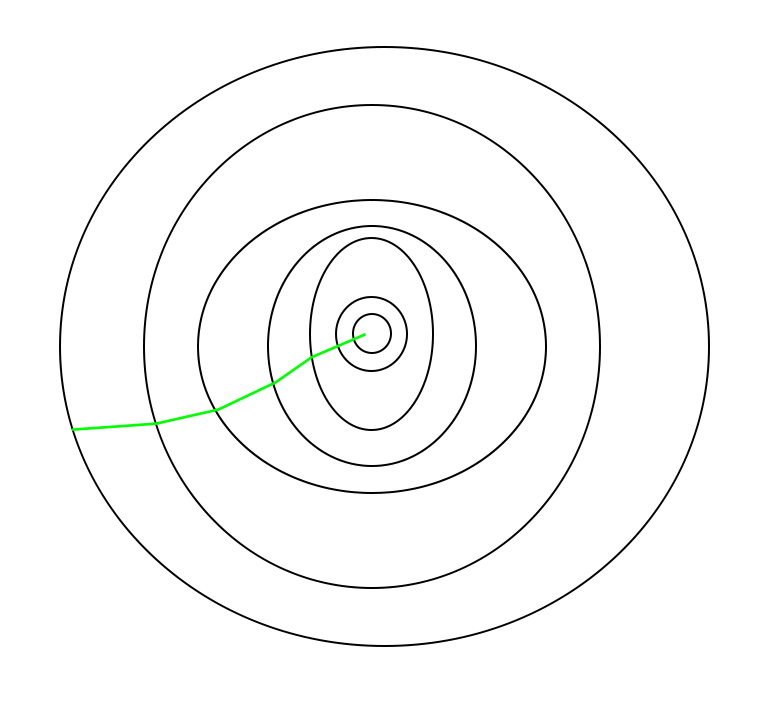
\includegraphics[width=5cm, height=5cm]{BGD.png}
\end{center}
A stochastic approach will result in noisy update rules, and will look something like that\\
\begin{center}

    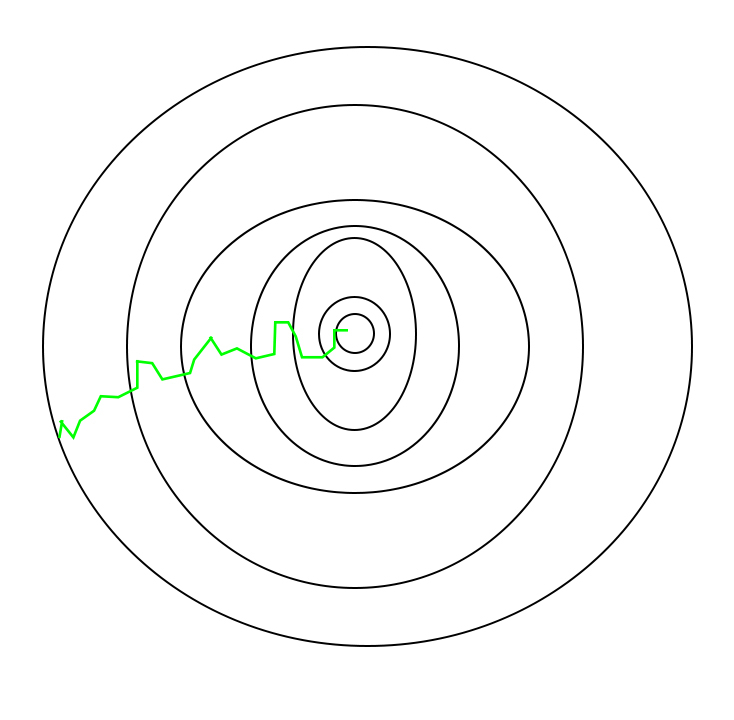
\includegraphics[width=5cm, height=5cm]{SGD.jpg}
\end{center}
The reason for choosing SGD over BGD is the fact that calculating the exact gradients of the objective function of each and every sample over an over until the convergence of the optimization process is extremely time consuming.
Considering working with large datasets (millions of data samples), using this method renders the optimization process almost unfeasible, thus the use of a stochastic approach is desired.

\section{Problem definition}

The most general formalism for optimization in supervised learning is as follows, let us denote $L(\theta)$ to be a noisy objective function, since it is a stochastic scalar function, and let it be differentiable w.r.t the parameters $\theta$. 
We want to find a mapping function $\hat{f}_\theta (x)$ that minimizes the objective function over all training samples:
$\min \limits_{\theta} \frac{1}{N}\sum_{i=1}^{N} L(y^i, \hat{f}_\theta (x^i))$. $L(\theta)$ 
, since it is a procedural optimization process that continues until convergence, we want to minimize the expected value of this function $\mathbf{E}[L_i(\theta)]$, with $L_1(\theta), ...L_T(\theta)$ being the realization of the function at subsequent timestamps 1,...,T.\\
Let $g=\nabla_\theta L_t(\theta)$ be the vector of partial derivatives of $f_t$, w.r.t $\theta$ evaluated at timestamp t. For the algorithm we will use 
\begin{equation*}
    m_t=\beta_1m_{t-1}+(1-\beta_1)g_t
\end{equation*}
which is the exponential moving average of the first moment of the gradient (mean) weighted with the parameter $\beta_1\in[0,1)$ and 
\begin{equation*}
    v_t=\beta_2v_{t-1}+(1-\beta_2)g^2_t
\end{equation*}
being the weighted average of the second moment of the gradient (the uncentered variance) with $\beta_2\in[0,1)$. $\beta_1$ and $\beta_2$ control the exponential decay rates of these moving
averages.
Both $m_t$ and $v_t$ are vectors initialized to zeros, which make the moments estimates to be biased towards zeros especially when the $\beta$s become closer to 1, so we need to fix them to be bias corrected, the resulting estimates are 
\begin{equation*}
    \begin{split}
    \hat{m}_t=\frac{m_t}{1-\beta_1^t} \\ 
    \hat{v}_t=\frac{v_t}{1-\beta_2^t}
    \end{split}
\end{equation*}

then we can use those moment estimates to update update the parameter $\theta$:
\begin{align*}
    \theta_{t+1}=\theta_t - \frac{\eta}{\sqrt{\hat{v_t}}+\eps}\hat{m_t}
\end{align*}
$\eta$ being the learning rate and $\eps$ is required to prevent numerical errors with very small standard deviations.
A pseudo-code of ADAM can be seen as follows:\\
\begin{center}
 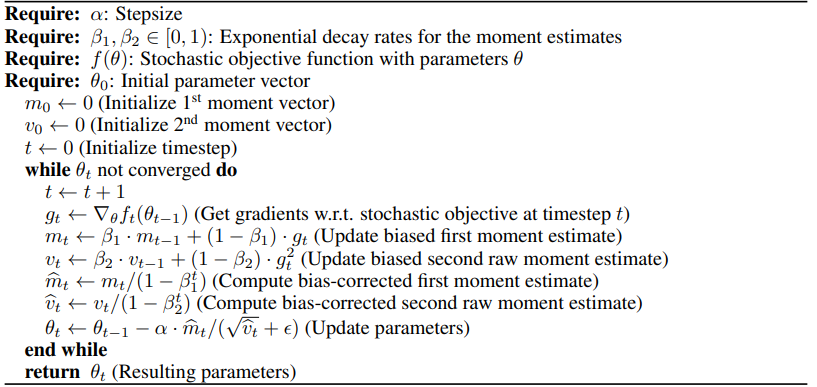
\includegraphics[scale=0.4]{pseudocode.png}
\end{center}

\section{Comparison to other optimizers and ADAM properties}
\textbf{Batch Gradient Descent} As mentioned in section 1, BGD passes through the whole dataset in batches, and store all the gradients in its path, lastly it performs the update step with fixed learning rate $\theta:=\theta-\eta \nabla_\theta L(\theta)$. \\
\textbf{Stochastic Gradient Descent} As we mentioned above vanilla SGD, is just apllying to each parameter the gradient of the error, with some learning rate, $\theta:=\theta-\frac{\eta}{n}\sum_{i=1}^{n}\nabla_\theta L_i(\theta;x_i,y_i)$. It is worth mentioning that almost all stochastic approach (including ADAM) have a notable quality that make them perform better on non-convex problems, the stochasity of the formulation makes it easy for them to stay away from local minimas, this also make them possibly miss the global minima or not converge exactly to it, especially in the case of SGD with a fixed learning rate. In the vanilla setup the error of convergence to a global minima in a covex setting of SGD is in the order of the learning rate, but if we add to vanilla SGD a learning rate schedule as suggested in \cite{darken1992learning} we can achieve the same optimal solution as in BGD.\\
\textbf{Mini batch Gradient Descent} is the combination of BGD and SGD, we do itterate over the all dataset in random batches, but update the parameters each batch, thus acheiving convergence much faster and still have the property of stochasity.
The key withdraw of all variants of gradient descent comparimg to ADAM (or other adaptive methods) is they use a learning rate which the user needs to wisely choose and is the same for all parameters, another key chalenge for those algorithms is saddle points, they do not perform well in smooth plateaus, which are common in deep learning \cite{dauphin2014identifying}.\\
As we mentioned earlier ADAM stands for adaptive moment estimation, the term adaptive refers to the property that ADAM calculates adaptive learning rates for each parameter, in contrast to SGD, in which the learning rate is fixed to all the parameters. This property is similar to other adaptive methods, such as Adadelta, Adagrad and RMSprop.\\
\textbf{Adagrad} is a gradient-based optimization algorithm that adapts the learning rate to the parameters, performing smaller updates for parameters associated with frequently occurring features, and larger updates (i.e. high learning rates) for parameters associated with infrequent features.\\
Let's denote $g_{t, i} = \nabla_\theta J( \theta_{t, i} )$, which is the partial derivative of the objective function w.r.t its parameters $\theta_i$, we calculate a diagonal matrix $G_t$, where each element is $G=\sum_{i=1}^{N} g_i g_i^T$, where N is the number of itterations, thus the update rule is $\theta_{t+1, i} = \theta_{t, i} - \dfrac{\eta}{\sqrt{G_{t, ii}} + \epsilon} \cdot g_{t, i}$
This method is well suited for sparse data because of its adaptivity to occurence of features.
\\
\textbf{Adadelta} 
\\
\textbf{RMSprop} was also introduced due to the shortcomings of Adagrad in regard to its quick decreasing of learning rate, it calculates the running average of past squared gradients $E[g^2]_t = \gamma E[g^2]_{t-1} + (1 - \gamma) g^2_t$, and the update rule is $\theta_{t+1} = \theta_{t} - \dfrac{\eta}{\sqrt{E[g^2]_t} + \epsilon} g_{t}$, we can see it is similar to the variance term in ADAM except the running average in RMSprop is only over the previous average of square gradients and ADAM is exponentially moving.
The other property of ADAM is moment estimation, ADAM calculates past gradient averages, similarly to momentum methods and in fact can be seen as a combination of a momentum method that does not calculate the variance and RMSprop that do not calculate the average, and lacks the term regarding the first moment averaging.\\
\textbf{AMSGrad} In \cite{reddi2019convergence} the authors argue that ADAM do not converge well to an optimal solution for convex problems, due to the exponential moving avergae of the gradients, which result in forgettness of long-term memory of past gradients. Therefor suggest an alternative AMSGrad which is a corrected version of ADAM, which replaces $\hat{v}_t$ to be $\hat{v}_t = \max(\hat{v}_{t-1}, v_t)$, all in all the authors get a similar algorithm to ADAM, but found that the de-biasing can be avoided, thus getting:
\begin{align} 
    \begin{split} 
    m_t &= \beta_1 m_{t-1} + (1 - \beta_1) g_t \\ 
    v_t &= \beta_2 v_{t-1} + (1 - \beta_2) g_t^2\\ 
    \hat{v}_t &= \text{max}(\hat{v}_{t-1}, v_t) \\ 
    \theta_{t+1} &= \theta_{t} - \dfrac{\eta}{\sqrt{\hat{v}_t} + \epsilon} m_t 
    \end{split} 
\end{align}
    
where $v_t$ is the regular moving average for the variance
this fixes the forgetness of ADAM and was shown to perform better on convex problems than ADAM, and we get an update rule similar to ADAM but never get an increasing step-size (which is to blame for its inability to converge).\\
Where ADAM shines is actually in non-convex error surface such as deep learning models (where it is widley used), and in \cite{chen2018convergence}, the authors even provided an upper bound for convergence rate under some mild conditions, but the authors showed that in some cases of deep learning problems AMSgrad outperforms ADAM.
\section{Miscellanea}
In \cite{vaswani2019painless}, the authors argue that althogh ADAM provide extremely good results on deep learning optimization i.e. trying to optimize a loss surface, it provide extremey poor results on other optimization problems.
The key difference between deep learning model optimization, is the shear number of parameters to optimize (several millions), and that derivatives of the error function are ususally ill conditioned \cite{li2017visualizing}, thus the error surface has many saddle points, thus from one hand convex optimization is not feasible in this cases, and in the other hand second order optimization is not feasible dus to the high dimensionality of parameters, which will require $O(n^2)$ in memory. This is where ADAM shines, it doesn't require more than calculating the gradients themselves, like SGD, but its momentum allows it to overcome local minima and saddle points, with its ability to properly tune the learning rate to different parameters.
\bibliography{proj}
\bibliographystyle{plain}
\end{document}

